% Options for packages loaded elsewhere
% Options for packages loaded elsewhere
\PassOptionsToPackage{unicode}{hyperref}
\PassOptionsToPackage{hyphens}{url}
%
\documentclass[
  11pt,
  letterpaper,
  DIV=11,
  numbers=noendperiod,
  twoside]{scrartcl}
\usepackage{xcolor}
\usepackage[left=1.1in, right=1in, top=0.8in, bottom=0.8in,
paperheight=9.5in, paperwidth=7in, includemp=TRUE, marginparwidth=0in,
marginparsep=0in]{geometry}
\usepackage{amsmath,amssymb}
\setcounter{secnumdepth}{3}
\usepackage{iftex}
\ifPDFTeX
  \usepackage[T1]{fontenc}
  \usepackage[utf8]{inputenc}
  \usepackage{textcomp} % provide euro and other symbols
\else % if luatex or xetex
  \usepackage{unicode-math} % this also loads fontspec
  \defaultfontfeatures{Scale=MatchLowercase}
  \defaultfontfeatures[\rmfamily]{Ligatures=TeX,Scale=1}
\fi
\usepackage{lmodern}
\ifPDFTeX\else
  % xetex/luatex font selection
  \setmainfont[ItalicFont=EB Garamond Italic,BoldFont=EB Garamond
Bold]{EB Garamond Math}
  \setsansfont[]{EB Garamond}
  \setmathfont[]{Garamond-Math}
\fi
% Use upquote if available, for straight quotes in verbatim environments
\IfFileExists{upquote.sty}{\usepackage{upquote}}{}
\IfFileExists{microtype.sty}{% use microtype if available
  \usepackage[]{microtype}
  \UseMicrotypeSet[protrusion]{basicmath} % disable protrusion for tt fonts
}{}
\usepackage{setspace}
% Make \paragraph and \subparagraph free-standing
\makeatletter
\ifx\paragraph\undefined\else
  \let\oldparagraph\paragraph
  \renewcommand{\paragraph}{
    \@ifstar
      \xxxParagraphStar
      \xxxParagraphNoStar
  }
  \newcommand{\xxxParagraphStar}[1]{\oldparagraph*{#1}\mbox{}}
  \newcommand{\xxxParagraphNoStar}[1]{\oldparagraph{#1}\mbox{}}
\fi
\ifx\subparagraph\undefined\else
  \let\oldsubparagraph\subparagraph
  \renewcommand{\subparagraph}{
    \@ifstar
      \xxxSubParagraphStar
      \xxxSubParagraphNoStar
  }
  \newcommand{\xxxSubParagraphStar}[1]{\oldsubparagraph*{#1}\mbox{}}
  \newcommand{\xxxSubParagraphNoStar}[1]{\oldsubparagraph{#1}\mbox{}}
\fi
\makeatother


\usepackage{longtable,booktabs,array}
\usepackage{calc} % for calculating minipage widths
% Correct order of tables after \paragraph or \subparagraph
\usepackage{etoolbox}
\makeatletter
\patchcmd\longtable{\par}{\if@noskipsec\mbox{}\fi\par}{}{}
\makeatother
% Allow footnotes in longtable head/foot
\IfFileExists{footnotehyper.sty}{\usepackage{footnotehyper}}{\usepackage{footnote}}
\makesavenoteenv{longtable}
\usepackage{graphicx}
\makeatletter
\newsavebox\pandoc@box
\newcommand*\pandocbounded[1]{% scales image to fit in text height/width
  \sbox\pandoc@box{#1}%
  \Gscale@div\@tempa{\textheight}{\dimexpr\ht\pandoc@box+\dp\pandoc@box\relax}%
  \Gscale@div\@tempb{\linewidth}{\wd\pandoc@box}%
  \ifdim\@tempb\p@<\@tempa\p@\let\@tempa\@tempb\fi% select the smaller of both
  \ifdim\@tempa\p@<\p@\scalebox{\@tempa}{\usebox\pandoc@box}%
  \else\usebox{\pandoc@box}%
  \fi%
}
% Set default figure placement to htbp
\def\fps@figure{htbp}
\makeatother


% definitions for citeproc citations
\NewDocumentCommand\citeproctext{}{}
\NewDocumentCommand\citeproc{mm}{%
  \begingroup\def\citeproctext{#2}\cite{#1}\endgroup}
\makeatletter
 % allow citations to break across lines
 \let\@cite@ofmt\@firstofone
 % avoid brackets around text for \cite:
 \def\@biblabel#1{}
 \def\@cite#1#2{{#1\if@tempswa , #2\fi}}
\makeatother
\newlength{\cslhangindent}
\setlength{\cslhangindent}{1.5em}
\newlength{\csllabelwidth}
\setlength{\csllabelwidth}{3em}
\newenvironment{CSLReferences}[2] % #1 hanging-indent, #2 entry-spacing
 {\begin{list}{}{%
  \setlength{\itemindent}{0pt}
  \setlength{\leftmargin}{0pt}
  \setlength{\parsep}{0pt}
  % turn on hanging indent if param 1 is 1
  \ifodd #1
   \setlength{\leftmargin}{\cslhangindent}
   \setlength{\itemindent}{-1\cslhangindent}
  \fi
  % set entry spacing
  \setlength{\itemsep}{#2\baselineskip}}}
 {\end{list}}
\usepackage{calc}
\newcommand{\CSLBlock}[1]{\hfill\break\parbox[t]{\linewidth}{\strut\ignorespaces#1\strut}}
\newcommand{\CSLLeftMargin}[1]{\parbox[t]{\csllabelwidth}{\strut#1\strut}}
\newcommand{\CSLRightInline}[1]{\parbox[t]{\linewidth - \csllabelwidth}{\strut#1\strut}}
\newcommand{\CSLIndent}[1]{\hspace{\cslhangindent}#1}



\setlength{\emergencystretch}{3em} % prevent overfull lines

\providecommand{\tightlist}{%
  \setlength{\itemsep}{0pt}\setlength{\parskip}{0pt}}



 


\setlength\heavyrulewidth{0ex}
\setlength\lightrulewidth{0ex}
\usepackage[automark]{scrlayer-scrpage}
\clearpairofpagestyles
\cehead{
  Brian Weatherson
  }
\cohead{
  The Asymmetric Magnets Problem
  }
\ohead{\bfseries \pagemark}
\cfoot{}
\makeatletter
\newcommand*\NoIndentAfterEnv[1]{%
  \AfterEndEnvironment{#1}{\par\@afterindentfalse\@afterheading}}
\makeatother
\NoIndentAfterEnv{itemize}
\NoIndentAfterEnv{enumerate}
\NoIndentAfterEnv{description}
\NoIndentAfterEnv{quote}
\NoIndentAfterEnv{equation}
\NoIndentAfterEnv{longtable}
\NoIndentAfterEnv{abstract}
\renewenvironment{abstract}
 {\vspace{-1.25cm}
 \quotation\small\noindent\emph{Abstract}:}
 {\endquotation}
\newfontfamily\tfont{EB Garamond}
\addtokomafont{disposition}{\rmfamily}
\addtokomafont{title}{\normalfont\itshape}
\let\footnoterule\relax
\KOMAoption{captions}{tableheading}
\makeatletter
\@ifpackageloaded{caption}{}{\usepackage{caption}}
\AtBeginDocument{%
\ifdefined\contentsname
  \renewcommand*\contentsname{Table of contents}
\else
  \newcommand\contentsname{Table of contents}
\fi
\ifdefined\listfigurename
  \renewcommand*\listfigurename{List of Figures}
\else
  \newcommand\listfigurename{List of Figures}
\fi
\ifdefined\listtablename
  \renewcommand*\listtablename{List of Tables}
\else
  \newcommand\listtablename{List of Tables}
\fi
\ifdefined\figurename
  \renewcommand*\figurename{Figure}
\else
  \newcommand\figurename{Figure}
\fi
\ifdefined\tablename
  \renewcommand*\tablename{Table}
\else
  \newcommand\tablename{Table}
\fi
}
\@ifpackageloaded{float}{}{\usepackage{float}}
\floatstyle{ruled}
\@ifundefined{c@chapter}{\newfloat{codelisting}{h}{lop}}{\newfloat{codelisting}{h}{lop}[chapter]}
\floatname{codelisting}{Listing}
\newcommand*\listoflistings{\listof{codelisting}{List of Listings}}
\makeatother
\makeatletter
\makeatother
\makeatletter
\@ifpackageloaded{caption}{}{\usepackage{caption}}
\@ifpackageloaded{subcaption}{}{\usepackage{subcaption}}
\makeatother
\usepackage{bookmark}
\IfFileExists{xurl.sty}{\usepackage{xurl}}{} % add URL line breaks if available
\urlstyle{same}
\hypersetup{
  pdftitle={The Asymmetric Magnets Problem},
  pdfauthor={Brian Weatherson},
  hidelinks,
  pdfcreator={LaTeX via pandoc}}


\title{The Asymmetric Magnets Problem\thanks{Thanks to the Philosophy
Program at the RSSS, ANU, where this was first drafted, to audiences at
University of Manitoba and Stanford University, and to the attendees at
my seminar on David Lewis at Cornell University. I am especially
grateful to Ben Caplan, John Hawthorne, Ishani Maitra, Raul Saucedo and
Wolfgang Schwarz.}}
\author{Brian Weatherson}
\date{2006}
\begin{document}
\maketitle
\begin{abstract}
There are many controversial theses about intrinsicness and duplication.
The first aim of this paper is to introduce a puzzle that shows that two
of the uncontroversial sounding ones can't both be true. The second aim
is to suggest that the best way out of the puzzle requires sharpening
some distinctions that are too frequently blurred, and adopting a fairly
radical reconception of the ways things are.
\end{abstract}


\setstretch{1.1}
There are many controversial theses about intrinsicness and duplication.
The first aim of this paper is to introduce a puzzle that shows that two
of the \emph{uncontroversial} sounding ones can't both be true. The
second aim is to suggest that the best way out of the puzzle requires
sharpening some distinctions that are too frequently blurred, and
adopting a fairly radical reconception of the ways things are.

\section{Two Theses about
Duplication}\label{two-theses-about-duplication}

In all of David Lewis's discussions of intrinsicness and duplication, he
held that the two concepts are connected by a tight circle of
interdefinition. Duplicates share all of their intrinsic features, and
objects that share all of their intrinsic features are duplicates.
(\citeproc{ref-Lewis1983e}{Lewis 1983b},
\citeproc{ref-Lewis1983b}{1983a};
\citeproc{ref-Lewis1998Langton}{Langton and Lewis 1998}). Both of these
claims are a little controversial. One might hold that some impure
properties that aren't shared by all duplicates, like \emph{having
George Clooney as a part}, are nevertheless intrinsic since gaining or
losing them seems to amount to a non-Cambridge change
(\citeproc{ref-Weatherson2006-WEAIVE}{Weatherson 2006}). And one might
hold that some properties which don't differ between duplicates by
definition, such as \emph{being a duplicate of the Louvre as it actually
is}, are nevertheless extrinsic (\citeproc{ref-Dunn1990}{Dunn 1990}). So
maybe Lewis's tight circle of interdefinition is not beyond question.
But the following principle seems utterly uncontroversial to me.

\textbf{Intrinsicness Principle}

\begin{itemize}
\tightlist
\item
  If \emph{a} and \emph{b} differ in their pure intrinsic features, they
  are not duplicates;
\item
  If \emph{a} and \emph{b} have the same pure intrinsic features, then
  they are duplicates
\end{itemize}

That conjunction is the first of our (hitherto) uncontroversial theses.
The second needs a bit more work to state formally.

It is fairly intuitive that whether two objects are duplicates is not an
emergent feature of reality. In some sense, whether two complex are
duplicates just depends on the properties of their parts and the
relations between their parts. But this claim \emph{does} turn out to be
controversial; David Lewis (\citeproc{ref-Lewis1983e}{1983b}) has
controverted it. To a first approximation, his theory says that whether
two objects are duplicates depends on whether they share the same
perfectly natural properties. If there are any perfectly natural
properties that are emergent, i.e.~which are properties that complex
objects have but \emph{not} in virtue of the properties of or relations
between their parts, then whether two objects are duplicates will also
be emergent. Now Lewis doesn't think there are any emergent perfectly
natural properties, since the existence of such properties would be
incompatible with the thesis of Humean Supervenience. But Lewis doesn't
think that Humean Supervenience is a necessary truth, let alone a
conceptual truth, but at best a contingent truth. So the principle that
duplication is not emergent is not something that is true in virtue of
the concept of duplication.

Still, nothing in Lewis's views suggest that the following principle is
false. If all the fundamental properties are not emergent, i.e.~they are
properties that complex things have in virtue of the fundamental
properties of and relations between their parts, then duplication is not
emergent. We might try and formalise this as follows. If all the
fundamental properties are not emergent, then if the parts of \emph{x}
and \emph{y} are duplicates, then \emph{x} and \emph{y} are duplicates.
This principle is, however, too strong. It doesn't account for the
possibility that the parts of \emph{x} and \emph{y} are arranged
differently. For instance, in the following example, the fusion of
\emph{a} and \emph{b} is not a duplicate of the fusion of \emph{c} and
\emph{d}, even though \emph{a} is a duplicate of \emph{c} and \emph{b}
is a duplicate of \emph{d}.

\pandocbounded{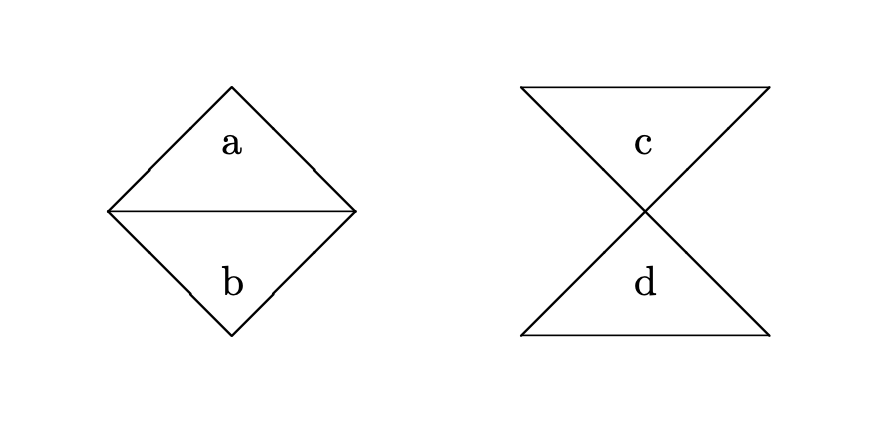
\includegraphics[keepaspectratio]{images/amp_1.png}}

The problem is that the arrangement of the two objects is different. So
what we need is a principle that says that if all the perfectly natural
properties are not emergent properties, and if the parts of \emph{x} and
\emph{y} are duplicates, and those parts are arranged the same way, then
\emph{x} and \emph{y} are duplicates. Saying this formally is not
exactly trivial. The following version uses the idea of an
isometry\footnote{An isometry is ``a transformation that does not change
  the distance between points'' (\citeproc{ref-Yaglom1962}{Yaglom 1962,
  11}). That is, it is a function from points to points that doesn't
  change distances. Although the isometry is initially defined as a
  function on points, it can obviously be extended to a function from
  regions to regions. If \emph{r} is a region, i.e.~a set of points,
  then \emph{f}(\emph{r}) is /\{\emph{f}(\emph{x}):
  \emph{x}~∈~\emph{r}/\}.}.

\textbf{Parts Principle}

\begin{quote}
This principle holds in all worlds in which no fundamental properties or
quantities are emergent. If X and Y are sets of material objects,
\emph{a} is the fusion of the members of X and \emph{b} is the fusion of
the members of Y, \emph{f} is a function X~→~Y, and \emph{i} is an
isometry defined on the space that X and Y are in, and the following
conditions hold:

\begin{itemize}
\tightlist
\item
  For all \emph{x} in X, \emph{f}(\emph{x}) is a duplicate of \emph{x};
  and
\item
  For all \emph{x} in X, if \emph{r} exactly occupied by \emph{x}, then
  \emph{i}(\emph{r})
\end{itemize}

is the region exactly occupied by \emph{f}(\emph{x}), then \emph{a} and
\emph{b} are duplicates.
\end{quote}

The Parts Principle is not as easy to state as the Intrinsicness
Principle, but I think the idea it is expressing is fairly intuitive.
Nevertheless, I think the two principles cannot both be true.

\section{Three Distinctions}\label{three-distinctions}

The problem I'll be focussing on looks rather simple, but it brings out
several points that seem to have metaphysical interest. In particular,
it highlights the importance of three distinctions that are easy to blur
when doing metaphysics. It will make the exposition of the puzzle easier
to place these distinctions up front.

The first distinction is between \emph{features} and \emph{properties}.
Most metaphysicians accept that to fully characterise the world, we need
to do more than say what exists. As well as saying what there is, we
need to say \emph{how} the things that exist are. It is easy to assume
that to do that, we need to say what properties things have. But this
need not be correct, or at least it need not be correct if we are
looking to characterise the world in the most fundamental way. It might
be that the fundamental features of reality are \emph{quantities},
i.e.~features that objects have to different degrees or in different
amounts. Properties, like \emph{being green} are features, but
quantities, like \emph{mass} or \emph{velocity} are also features, just
features that can be instantiated to different degrees or magnitudes. So
\emph{feature} is a more general category than \emph{property}, and so
as to not beg any questions, I'll talk about intrinsic features and
fundamental features rather than intrinsic properties and fundamental
properties throughout. My solution to the problem will involve assuming
that at least some of the fundamental features of reality are indeed
quantities not properties.

The second distinction is between \emph{fundamental} features and
\emph{perfectly natural} features. Fundamental features are features
that do not obtain in virtue of other features obtaining. The
fundamental features are part of a minimal basis we need for
characterising reality. Generally fundamental features are related to
other fundamental features by exceptionless laws, though this is not
part of their definition. What is definitional is that they are basic
and that they provide a basis for characterising the world without
redundancy. (As a Humean, I'd also say that there are no necessary
connections between distinct fundamental features, but that is a
controversial metaphysical thesis, not a defining characteristic.)
Perfectly natural features are features that make for primitive
objective resemblance between things that instantiate them. By a
\emph{primitive} objective resemblance, I mean an objective resemblance
that does not obtain in virtue of sharing more basic (in the limit,
fundamental) properties. David Lewis (\citeproc{ref-Lewis1983e}{1983b})
assumes, without much by way of argument as far as I can see, that the
fundamental features are the perfectly natural features. My solution to
the problem will involve rejecting that identity.

The final distinction is between the thesis that all the fundamental
non-spatiotemporal features of reality are intrinsic properties of
points, and the thesis that these features are \emph{local} features.
Jeremy Butterfield (\citeproc{ref-Butterfield2006}{2006}) has stressed
the importance of this distinction for metaphysics. A feature is local
to a point iff it is intrinsic to arbitrarily small regions around that
point. For example, the slope of a curve at a point is local to that
point, even though it isn't intrinsic to the point. So locality and
intrinsicness can come apart. (This raises interesting questions about,
for example, whether it is best to state the thesis of Humean
Supervenience in terms of local properties or in terms of intrinsic
properties of points.) I'll say more about the importance of this
distinction in section 5.

I've already made use of these distinctions in setting out the
principles about intrinsicness in section one. (In particular, it is
crucial that the Parts Principle is stated in terms of
\emph{fundamental} rather than \emph{perfectly natural} features.) Using
them we can get to our central puzzle, the Asymmetric Magnets Problem.

\section{The Asymmetric Magnets
Problem}\label{the-asymmetric-magnets-problem}

Our puzzle is similar to the spinning sphere, often thought to raise a
problem for Humean Supervenience (\citeproc{ref-Armstrong1980}{Armstrong
1980}). The similarity is not in respect of its target; the puzzle is
meant to be a puzzle for everyone who accepts those two principles, not
just the Humean. Rather, the similarity is in that the puzzle is set in
a world where there are homogeneous physical objects. Such a world is in
many ways quite distant from actuality. But I think such worlds are
useful fictions for elucidating the conceptual connections between
central concepts in metaphysics. The puzzle is also set in a world with
Euclidean spatial geometry. Again this is a fiction, but a useful one
for working out conceptual connections.

In this world, some of the fundamental features are what we'll call
\emph{vector features}. (This is a much smaller deviation from
actuality.) Vector features are either quantities like \emph{velocity}
the value of which is a vector, or properties like \emph{having
velocity} \emph{v}, where \emph{v} is some vector. In particular, the
strength and direction of the magnetic field throughout the world is a
fundamental feature of the world. I'll assume that both space-time
regions and physical objects can have these vector features, although
I'm only going to focus on the field strength and direction at a point
in a physical object. Finally, I'll assume that all of the fundamental
physical quantities in the world are local. So there are no fundamental
emergent quantities in the world. It might be worried that the last two
assumptions are inconsistent, and that vector quantities could not be
local. I'll come back to this worry in section 5.

Some of the things in this world are \emph{magnets}. These are
homogeneous objects with a uniform non-zero magnetic field throughout.
I'm going to represent the magnetic field strength and direction of such
a magnet with an arrow pointing towards the north pole of the magnet.
The length of the arrow is proportional to the strength of the field.

The simplest kind of magnet is a bar magnet, just like the kind I used
to play with in primary school. (Apart from being homogeneous of
course!) These are cuboids with equal heights and depths, and a long
length in the direction of their magnetic field. Suzy is playing with
some magnets and, tiring of using her magnets to grab the other
childrens', decides to sharpen one end of each of her magnets for use as
a weapon. The teacher notices this, confiscates the weaponised magnets,
and lays them out on her desk. Here is what they look like from the
teacher's point of view.

\pandocbounded{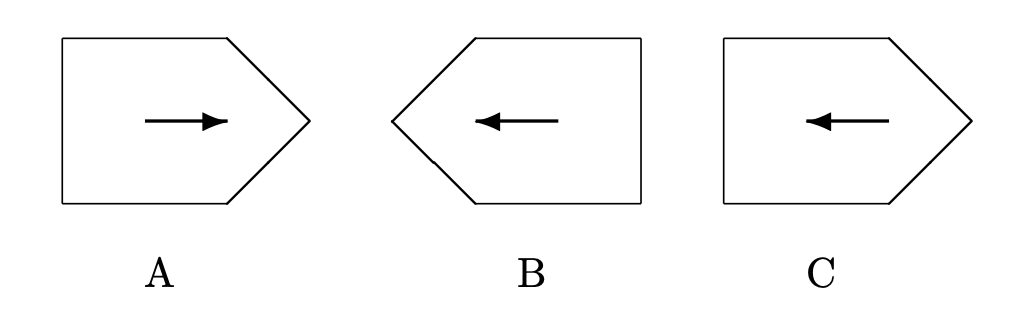
\includegraphics[keepaspectratio]{images/amp_2.png}}

I've added the labels.

Each magnet has one sharp end and one flat end. Each also has one north
pole and one south pole. And, of course, each has one end to the right
(from the teachers' point of view) and one end to the left. The
distribution of these properties of ends is different in the three
cases.

\begin{itemize}
\tightlist
\item
  A's north pole is sharp and to the right.
\item
  B's north pole is sharp and to the left.
\item
  C's north pole is flat and to the left.
\end{itemize}

Question: Which of the magnets are duplicates?

Answer: A and B, but not C.

I hope you agree with the answer! If not, let me provide a small
argument.

A and B are intrinsic duplicates because we could `line up' A and B by
picking A up, spinning it around, and moving it across a bit. And that's
only possible if the two objects are duplicates. This idea, that objects
that can be transformed into one another by simple geometric
transformations such as rotation and translation is a very deep part of
our conceptual scheme. Consider, for example, Euclid's proof of
proposition 4.

\begin{quote}
Let \emph{ABC}, \emph{DEF} be two triangles having the two sides
\emph{AB}, \emph{AC} equal to the two sides \emph{DE}, \emph{DF}
respectively, namely \emph{AB} to \emph{DE} and \emph{AC} to \emph{DF},
and the angle \emph{BAC} equal to the angle \emph{EDF}. I say that the
base \emph{BC} is also equal to the base \emph{EF}, the triangle
\emph{ABC} will be equal to the triangle \emph{DEF} \ldots{} For, if the
triangle \emph{ABC} be applied to the triangle \emph{DEF}, and if the
point \emph{A} be placed on the point \emph{D} and the straight line
\emph{AB} on \emph{E}, then the point \emph{B} will also coincide with
\emph{E}, because \emph{AB} is equal to \emph{DE}. Again, \emph{AB}
coinciding with \emph{DE}, the straight line \emph{AC} will also
coincide with \emph{DF}, because the angle \emph{BAC} is equal to the
angle \emph{EDF}; hence the point \emph{C} will also coincide with the
point \emph{F}, because \emph{AC} is again equal to \emph{DF}. But
\emph{B} also coincided with E; hence the base \emph{BC} will coincide
with the base \emph{EF} \ldots{} and will be equal to it. Thus the whole
triangle \emph{ABC} will coincide with the whole triangle \emph{DEF},
and will be equal to it. (\citeproc{ref-Euclid1956}{Euclid 1956,
247--48})
\end{quote}

As many mathematicians have pointed out over the centuries, this is not
Euclid's finest moment as a geometer. The idea he's pushing is clear
enough. If \emph{ABC} and \emph{DEF} satisfy the assumptions, then you
can pick up \emph{ABC} and place it on \emph{DEF}, so that the sides and
vertices all coincide. Does this prove that the sides and angles in the
original triangle are equal? Not really, or at least not without the
assumption that picking up \emph{ABC} and moving it around doesn't
change its side lengths or angle magnitudes. And Euclid hadn't said
anything at that stage of the \emph{Elements} to justify this
assumption.

So \emph{qua} axiomatic geometer Euclid has blundered here. But there is
more to life than axiomatic geometry. There is, for instance,
metaphysics. And the assumption Euclid is using here is, I think, a
sound metaphysical intuition. (If it weren't, the complaints about this
fundamental proof in Euclid would have been earlier, and more frequent,
than they actually were.) That intuition is, I think, that intrinsic
properties are not, ceteris paribus, changed merely by moving objects
around. Of course other things are not always equal; the intrinsic
properties of a car are not preserved if you drive it into a wall. But
the kind of abstract motion that Euclid is contemplating when he moves
\emph{ABC} onto \emph{DEF}, or that I'm contemplating when I think about
moving B around so it lines up with A, does not destroy intrinsic
properties. So that's an argument that A and B are intrinsically alike.

On the other hand, A and B each have a property that C lacks. Their
magnetic field points towards their sharp end. This is in some sense a
relational property, it is defined in part in terms of two things
pointing in the same direction, but it doesn't seem like a relation
between the magnet and anything else. In general, properties that things
have in virtue of relations between their parts are intrinsic
properties. (It is intrinsic to the earth, for example, that more of its
surface is wet than dry, even though this property is defined in terms
of a relation.) So this is an intrinsic property of A. And, given the
plausibility of the Intrinsicness Principle, that's a reason to think
that A and C are not intrinsic.

\section{The Principles and the
Problem}\label{the-principles-and-the-problem}

Here then is our problem. Try to answer the following question given the
two principles: Is the direction of a vector feature an intrinsic
feature of its bearer or not? If yes, then A and B are not duplicates.
If no, then A and C are duplicates. (In fact all three are duplicates,
though I won't prove this.) Neither way does it turns out that A and B
are duplicates, but C is not, as we need. The aim of this section is to
spell out that little argument in more detail, so we can see how the
principles relate to the problem.

First, we'll assume that the direction of a vector feature is an
intrinsic feature of its bearer. We need a way to rigidly denote
directions, so we'll call the direction that the vector in \emph{A}
points \emph{d}\textsubscript{1}, and the direction that the vector in
\emph{B} points \emph{d}\textsubscript{2}. Since
\emph{d}\textsubscript{1}~≠~\emph{d}\textsubscript{2}, \emph{A} and
\emph{B} differ in their intrinsic properties. By the second clause of
the Intrinsicness Principle, it follows that \emph{A} and \emph{B} are
not duplicates.

Second, we'll assume that the direction of a vector feature is not an
intrinsic feature of its bearer. Now we want to show that B and C are
duplicates. To do this we'll use the Parts Principle. All of the
fundamental quantities are local, so the Parts Principle applies. Now
let the members of X and Y be the point-sized parts of A and C. Let
\emph{l} be the distance from the tip of the pointed end of A to the tip
of the pointed end of C. The isometry \emph{i} is a translation with
length \emph{l} and direction \emph{d}\textsubscript{1}, i.e.~a function
that maps any point to the point that is distance \emph{l} away from it
in direction \emph{d}\textsubscript{1}. This isometry maps A onto C. By
the first clause of the Intrinsicness Principle, and the assumption that
direction is not intrinsic, every point in A is a duplicate of any point
in C. So by the Parts Principle, A and C are required.

The conclusion is that if we want to say that A and B are duplicates,
but A and C are \emph{not} duplicates, then we can't hold on to both the
Intrinsicness Principle and the Parts Principle.

I think we should give up the Parts Principle. In particular, we should
say that the Parts Principle holds only if all the \emph{perfectly
natural} features of reality are local, and this might fail to hold even
if all the \emph{fundamental} features of reality are local. The need
for the distinction between these possibilities is, I think, the main
lesson of the problem. But before we get to that conclusion, I want to
address an objection to the argument so far.

\section{Two Worries About Locality}\label{two-worries-about-locality}

I can an imagine an objection to this argument along the following
lines. In the setup of the problem, I said that some of the fundamental
features of reality are vector-valued quantities. I also said that all
of the fundamental features of reality are local. But these assumptions
are inconsistent. Vector properties are not intrinsic properties of
points. (Since we're trying to hold on to the Intrinsicness Principle,
we have to accept this.) Hence they are not, in the salient sense, local
features of reality.

I think this objection is sound all the way to the last step. As noted
above, we need to distinguish between local properties and intrinsic
properties of points. The distinction is common in mathematics, but has
not been paid sufficient attention in metaphysics. Jeremy Butterfield's
(\citeproc{ref-Butterfield2006}{2006}) is an important exception, one
that was very influential on this paper.

So it is fair to say that all fundamental features of reality are local
if all the facts about the world supervene on facts about the
distribution of fundamental features in arbitrarily small regions, plus
facts about the spatiotemporal arrangement of those regions. And there
is no reason to think that positing vector features as fundamental is
inconsistent with the fundamental features being local in this sense.
Butterfield argues, persuasively, that velocity properties in Newtonian
mechanics are not intrinsic properties of points, but he stresses that
this doesn't mean they are not local in this sense. He is focussing on
velocity, and what he says doesn't \emph{immediately} translate to all
vector properties. (It matters to his argument, for example, that
velocities are conceptually connected to the positions of objects
\emph{at different times}, in a way that, for example, magnetic fields
are not.) But I think his conclusions are independently plausible.
Indeed, the argument from isometry above is an argument for the very
same conclusion. So the short version of my reply is to concede that
once we've allowed vector properties as fundamental, we can't say that
all the fundamental features of reality are intrinsic properties of
points and spatiotemporal relations between them, but this is consistent
with saying that all the fundamental features of reality are local.

Once we've said that, however, a different kind of objection becomes
salient. It might be thought that if the fundamental features are
intrinsic properties of regions not of points, the natural version of
the Parts Principle is slightly weaker than as stated. In particular, we
should focus our attention to cases where the sets X and Y consist of
objects with positive size. Because this weakening flows naturally from
the definition of locality, it doesn't look like an \emph{ad hoc}
weakening. However this weakening does not at the end of the day help to
save the Parts Principle. That's because we can find a different way to
divide up A and C into parts of positive size so that the Parts
Principle still applies. A sketch of how we'll (start to) divide up A is
here.

\pandocbounded{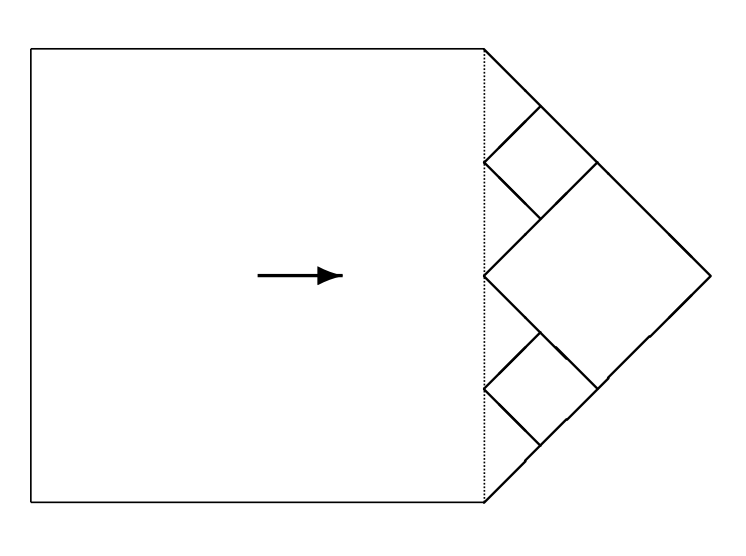
\includegraphics[keepaspectratio]{images/amp_3.png}}

The idea is that we make one large square part, and then divide the rest
of A up into infinitely many diamonds. We do this recursively. Note that
we start with a triangle whose base is to the left and vertex to the
right. We create from this a diamond whose four vertices are the vertex
of the triangle, and the midpoints of each of the three sides of the
triangle. If we imagine cutting this diamond out of the magnet, we'd be
left with two small triangles, each with a base on the left and a vertex
on the right. We can do the same trick to create diamonds and (in
imagination) cut them out, leaving us with four triangles. Repeat this
until we have an infinity of diamonds. The fusion of all these diamonds
with the large square will be our original magnet. Moreover, since every
part is symmetric around the axis perpendicular to
\emph{d}\textsubscript{1}, each part will be a duplicate of the
corresponding part in C. So the Parts Principle still tells us, falsely,
that A and C are duplicates. We have to look somewhere else to avoid the
problem.

\section{The solution and its
problems}\label{the-solution-and-its-problems}

The Asymmetric Magnets Problem looks easy. It is easy to say intuitively
why A and B are duplicates, but C is not. The reason was given at the
end of section three. In both A and B, the magnetic field `points' in
the same direction that the physical object does, while in C this is not
the case. The difficulty arises when we try and shoehorn this intuition
into a formal theory. We need to say that it is intrinsic to the magnet
that its magnetic field points the same way it does. And we need to say
this without saying that the direction of the magnetic field is itself
intrinsic. I know of one way to do this, but it involves some overheads.
I'm not going to argue for this at any length here, but I think the
difficulty of providing a general solution to the Asymmetric Magnets
Problem is one of many reasons to think that we should learn to live
with these overheads.

My solution starts with Lewis's definition of duplication. I gave a
rough statement of this above; we now need a more precise statement. For
Lewis, two objects are duplicates iff there is a mapping \emph{m} from
parts of one to parts of the other that (a) is an isomorphism and (b)
for all \emph{n}-place perfectly natural properties \emph{P}, and all
parts \emph{x}\textsubscript{1}, \ldots, \emph{x\textsubscript{n}} of
the first object,
\emph{Px}\textsubscript{1}\ldots{}\emph{x\textsubscript{n}} iff
\emph{Pm}(\emph{x}\textsubscript{1})\ldots{}\emph{m}(\emph{x\textsubscript{n}}).
So the objects are duplicates if their parts have the same natural
properties, and stand in the same perfectly natural relations. That's
how Lewis's theory goes; now we have to start adding variations. The
first variation is quite radical, but one we have independent reason to
make.

As John Hawthorne (\citeproc{ref-Hawthorne2006}{2006}) and David Denby
(\citeproc{ref-Denby2001}{2001}) have argued, Lewis's theory of
properties has difficulties accounting for \emph{quantities}. Hawthorne
notes that if we just take individual mass properties, e.g.~\emph{having
mass 17kg}, \emph{having mass 42ng} etc as perfectly natural, there is
no way to state physical laws involving mass, such as the law of
gravitation, as simple statements where all predicates denote perfectly
natural properties. But the theory of laws in Lewis
(\citeproc{ref-Lewis1983e}{1983b}) says that all physical laws
\emph{are} simple statements where all predicates denote perfectly
natural properties. This is something of a problem. For different
reasons, Denby suggests that we take \emph{determinables} as being
perfectly natural. The individual mass properties are perfectly natural,
he suggests, but not fundamental. What is fundamental is the
determinable, \emph{mass}, of which they are determinate.

I think we should make a more radical move in the interests of
simplicity. What reason do we have for thinking that the fundamental
ways things are are \emph{properties} rather than \emph{quantities} or
\emph{magntitudes}? Very little reason, I'd say. Modern physics seems
much more concerned with quantities than properties. What properties it
is concerned with, such as \emph{being positively charged}, seem to be
derived from more fundamental quantities, such as charge. It would
perhaps be convenient for formal semantics if the world had an
object-property structure to match the subject-predicate structure of
simple sentences. But we have no reason to believe the world will be so
accommodating. It might turn out that there are a few fundamental
\emph{quantities} in the world. A quantity is a feature that objects
have to different degrees. We can identify each value a quantity takes
with a property. (Examples are properties like \emph{having mass 17kg}.)
But that shouldn't make us think that the properties are metaphysically
primary. They might be derived from the quantities. Hawthorne's and
Denby's arguments push us towards that conclusion, and I'll show here
that assuming quantities are primary helps us state a solution to the
Asymmetric Magnets Problem.

Some quantities take simple values. The values of the \emph{mass}
quantity, for instance, are sufficiently simple that they can be
represented by real numbers. But not all quantities are like that. In
some cases the values are structured entities, which are composed of a
magnitude and some other some other part or parts. Vector quantities are
like this. We can naturally think of vectors as structured entities
composed of a direction and a magnitude. I'm going to assume, at least
for the sake of solving this problem, that any perfectly natural
quantity takes values that either are magnitudes (as \emph{mass} does)
or takes values that are structured entities composed, among other
things, of a magnitude. (This is an empirical assumption, and it may
well not be true. If it is not true, the analysis of duplication below
will need to be made more complicated.) For ease of exposition, I'll say
that a function \emph{f} is perfectly natural iff it maps objects onto
values, such that there is some perfectly natural quantity such that for
any \emph{x}, \emph{f}(\emph{x}) is the value that quantity takes with
respect to \emph{x}. So if the quantity is mass, \emph{f}(\emph{x}) is
\emph{x}'s mass. And I'll say that
\textbar{}\emph{f}(\emph{x})\textbar{} is the \emph{magnitude} of this
value, in the sense described above. (The notation here is slightly
non-standard, since I allow that magnitudes may be negative numbers. For
example, if \emph{f} represents charge and \emph{x} is negatively
charged, then \textbar{}\emph{f}(\emph{x})\textbar{} may be a negative
number.)

Now for the definition of duplication. Two objects are duplicates iff
there is a mapping \emph{m} from parts of one to parts of the other that
(a) is an isomorphism and (b) for all \emph{n}-place natural functions
\emph{f}, and all parts \emph{x}\textsubscript{1}, \ldots,
\emph{x}\textsubscript{n} of the first object,
\textbar{}\emph{f}(\emph{x}\textsubscript{1},\ldots,
\emph{x}\textsubscript{n})\textbar{} =
\textbar{}\emph{f}(\emph{m}(\emph{x}\textsubscript{1})),\ldots,\emph{f}(\emph{m}(\emph{x}\textsubscript{n}))\textbar.
So the objects are duplicates if the magnitudes of each of the natural
quantities of each of their parts are the same. This allows that the
quantities can vary without loss of intrinsic character, provided there
is no variation in magnitude.

The Asymmetric Magnets Problem suggests a view on which the directions
of vector features are \emph{indirectly relevant} to the intrinsic
nature of objects. `Indirectly' because changing the direction doesn't
change the intrinsic properties of objects. But `relevant' because the
direction can matter, as we see when comparing A and C. The definition
of duplication in terms of quantities that take structured values allows
us to capture this indirect relevance. We'll do so by defining a feature
whose magnitude varies depending on how the object's shape and the
direction of its vector features are coordinated.

Let \emph{f} be a function representing some perfectly natural quantity
such that \emph{f}(\emph{x}) is a vector. That is, \emph{f} represents
some perfectly natural vector quantity. This quantity may or may not be
fundamental, though it will be fundamental in the cases under
consideration here. Let \emph{c} be a function that takes an object as
input and returns its geometric centre as output. (By the geometric
centre of \emph{x} I mean the centre of mass of an object with the same
shape as \emph{x} and uniform mass density throughout.) Now suppose that
the following function is perfectly natural.

\begin{quote}
\emph{g}(\emph{x}, \emph{y}, \emph{z}) =\textsubscript{df} the cosine of
the angle between \emph{f}(\emph{x}) and the ray from \emph{g}(\emph{y})
to \emph{g}(\emph{z}).
\end{quote}

The motivation for taking this to be perfectly natural (but obviously
not fundamental) is that it delivers the right results about the
Asymmetric Magnets Problem, and it seems to deliver those results for
the right reasons. To see it delivers the right results, just apply the
above definition of duplication. Two objects are duplicates iff there is
an isomorphism \emph{m} from the parts of one to the parts of the other
such that for all \emph{n}-place natural functions \emph{f}, and all
parts \emph{x}\textsubscript{1}, \ldots, \emph{x}\textsubscript{n} of
the first object, \textbar{}\emph{f}(\emph{x}\textsubscript{1},\ldots,
\emph{x}\textsubscript{n})\textbar{} =
\textbar{}\emph{f}(\emph{m}(\emph{x}\textsubscript{1})), \ldots,
\emph{f}(\emph{m}(\emph{x}\textsubscript{n}))\textbar. To make the
discussion easier, we'll redraw the magnets with some salient parts
labelled.

\pandocbounded{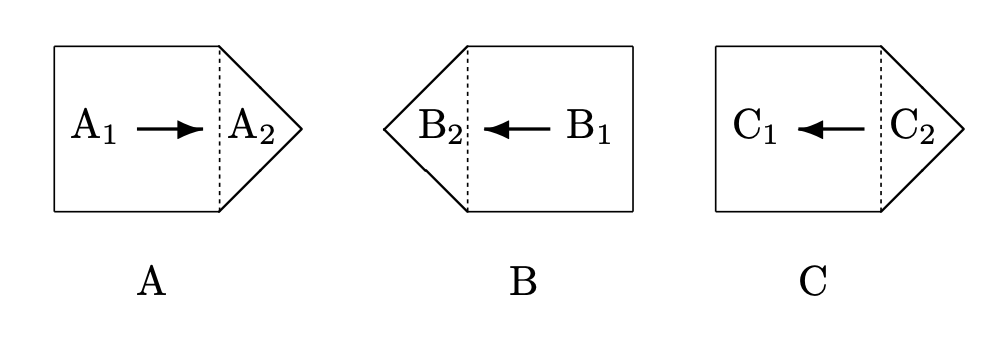
\includegraphics[keepaspectratio]{images/amp_4.png}}

Any isomorphism from A to B that satisfy this constraint has to map
A\textsubscript{1} to B\textsubscript{1}, and A\textsubscript{2} to
B\textsubscript{2}. And any isomorphism from A to C that satisfy this
constraint has to map A\textsubscript{1} to C\textsubscript{1}, and
A\textsubscript{2} to C\textsubscript{2}. Now let \emph{f} be the
function whose value is represented by the arrow, and let \emph{g} be
the function defined as above. So if A and B are duplicates, it must be
the case that \emph{g}(A, A\textsubscript{1}, A\textsubscript{2}) =
\emph{g}(B, B\textsubscript{1}, B\textsubscript{2}). It is easy to
verify that since \emph{f}(A) points in the same direction as the ray
from the centre of A\textsubscript{1} to the centre of
A\textsubscript{2}, \emph{g}(A), A\textsubscript{1}, A\textsubscript{2}
= 1, and similarly the ray from the centre of B\textsubscript{1} to the
centre of B\textsubscript{2} points in the same direction as
\emph{f}(B), \emph{g}(B, B\textsubscript{1}, B\textsubscript{2}) = 1. So
there is no reason here to doubt that A and B are duplicates. On the
other hand, since the ray from the centre of C\textsubscript{1} to the
centre of C\textsubscript{2} is in the opposite direction to
\emph{f}(C), \emph{g}(C, C\textsubscript{1}, C\textsubscript{2}) = -1.
So there is no isomorphism from parts of A to parts of C that preserves
the value of perfectly natural properties, so A and C are not
duplicates, as required.

I don't doubt that there are other ways to solve this problem, so I
certainly won't try arguing that this is the only solution. But I think
it works, and the reason it works is because the values of natural
quantities are structured entities, in this case vectors. Because they
have structure, we can use one part of the structure (i.e.~the
magnitude) in determining what is directly relevant to intrinsicness,
and another part of the structure (in this case the direction) in
determining what is indirectly relevant. So it's an important advantage
of using quantities rather than properties as the centrepiece of our
metaphysics that the values of natural quantities can be structured
entities, and having something like structured quantities seems crucial
to solving this problem.

Although \emph{g} is represents a perfectly natural quantity, it does
not represent a \textbf{fundamental} quantity. Instead, it represents a
quantity whose value supervenes on the distribution of other perfectly
natural quantities. So we have to allow that there is a distinction
between the fundamental quantities and the perfectly natural quantities.
I don't think this is a cost of the theory; there is no way to capture
the idea that directions are indirectly relevant without distinguishing
between the perfectly natural and the fundamental, so the Asymmetric
Magnets Problem is a reason to make such a distinction. (I'm indebted
here to Ben Caplan.)

We can reduce the apparent cost of this distinction by noting that one
reason we might have for blocking redundant natural quantities does not
apply here. (By a redundant quantity, I just mean one that supervenes on
the fundamental quantities.) We don't want to say that
\emph{disjunctive} properties like \emph{being grue}, that supervene on
other natural properties, are perfectly natural. But that's not
primarily because of the supervenience, but because of the fact that
grueness doesn't make for resemblance amongst the things that
instantiate it. So at least that reason for caring about redundancy
doesn't apply here. (I'm indebted here to Raul Saucedo.)

Finally, it is crucial to my solution that A, B and C have these parts.
If A, B and C are extended simples, I can't run the argument I make
here. Indeed, if they are extended simples, it looks like they are
duplicates by my definition. That seems bad. I think this is a problem
that we don't need to worry about, because this isn't a real
possibility. I'll concede for the sake of argument that there are such
things as extended simples. What I don't see any need to concede the
possibility of are \emph{asymmetric} extended simples. In general, the
way that we deduce that an object has parts is by noting it has
different properties at different places. (This point is made in Sider
(\citeproc{ref-Sider2003}{2003}).) I think this is just the right
strategy to use, as a matter of necessity. If an object has different
properties in different locations, it has different parts in those
different locations. So there could not be extended simples that are
\emph{asymmetric} magnets. The case where my theory produces the wrong
result is an impossible case.

\section{Wrapping Up}\label{wrapping-up}

This paper has had several ambitions, some loftier than others. The most
basic aim has been to introduce the Asymmetric Magnets Problem, and
argue that it is going to be hard work for a systematic theory of
intrinsicness to account for the facts about the problem. The more
profound aims involve tearing apart concepts that metaphysicians often
take for granted are interchangeable. My solution to the problem
involves distinguishing local features from intrinsic features of
points, fundamental features from perfectly natural features, and, most
importantly, features from properties. The last of these is I think the
biggest point. If we come to believe that quantities, not qualities, are
the fundamental ways things are, then quite a bit of metaphysical
orthodoxy needs rewriting. Some of that rewriting may be simple; just a
matter of crossing out `li' and writing in `nt' in the middle of some
words. But changes in fundamental metaphysics tend not to be isolated,
and the rewriting project may lead to more wide-ranging changes. (Egan
(\citeproc{ref-Egan2004-JACSPA-2}{2004}) makes this point well, with an
important illustration.) Now I certainly haven't given anything like a
conclusive argument in this paper that we should set about that project
immediately. I have, however, provided one reason to think the project
will eventually be necessary, and I suspect that more reasons will be
provided in the future.

\subsection*{References}\label{references}
\addcontentsline{toc}{subsection}{References}

\phantomsection\label{refs}
\begin{CSLReferences}{1}{0}
\bibitem[\citeproctext]{ref-Armstrong1980}
Armstrong, David. 1980. {``Identity Through Time.''} In \emph{Time and
Cause: Essays Presented to Richard Taylor}, edited by Peter van Inwagen,
67--78. Dordrecht: Reidel.

\bibitem[\citeproctext]{ref-Butterfield2006}
Butterfield, Jeremy. 2006. {``Against Pointillisme about Mechanics.''}
\emph{British Journal for the Philosophy of Science} 57 (4): 709--53.
doi: \href{https://doi.org/10.1093/bjps/axl026}{10.1093/bjps/axl026}.

\bibitem[\citeproctext]{ref-Denby2001}
Denby, David. 2001. {``Determinable Nominalism.''} \emph{Philosophical
Studies} 102 (3): 297--327. doi:
\href{https://doi.org/0.1023/A:1010314926955}{0.1023/A:1010314926955}.

\bibitem[\citeproctext]{ref-Dunn1990}
Dunn, J. Michael. 1990. {``Relevant Predication 2: Intrinsic Properties
and Internal Relations.''} \emph{Philosophical Studies} 60 (3):
177--206. doi:
\href{https://doi.org/10.1007/bf00367469}{10.1007/bf00367469}.

\bibitem[\citeproctext]{ref-Egan2004-JACSPA-2}
Egan, Andy. 2004. {``Second-Order Predication and the Metaphysics of
Properties.''} \emph{Australasian Journal of Philosophy} 82 (1): 48--66.
doi: \href{https://doi.org/10.1080/713659803}{10.1080/713659803}.

\bibitem[\citeproctext]{ref-Euclid1956}
Euclid. 1956. \emph{The Thirteen Books of the Elements, {Tr. Thomas l.
Heath}}. New York: Dover.

\bibitem[\citeproctext]{ref-Hawthorne2006}
Hawthorne, John. 2006. {``Quantity in Lewisian Metaphysics.''} In
\emph{Metaphysical Essays}, 229--37. Oxford: Oxford University Press.

\bibitem[\citeproctext]{ref-Lewis1998Langton}
Langton, Rae, and David Lewis. 1998. {``Defining {`Intrinsic'}.''}
\emph{Philosophy and Phenomenological Research} 58 (2): 333--45. doi:
\href{https://doi.org/10.2307/2653512}{10.2307/2653512}. Reprinted in
his \emph{Papers in Metaphysics and Epistemology}, Cambridge: Cambridge
University Press, 1999, 116-132. References to reprint.

\bibitem[\citeproctext]{ref-Lewis1983b}
Lewis, David. 1983a. {``Extrinsic Properties.''} \emph{Philosophical
Studies} 44 (2): 197--200. doi:
\href{https://doi.org/10.1007/bf00354100}{10.1007/bf00354100}. Reprinted
in his \emph{Papers in Metaphysics and Epistemology}, Cambridge:
Cambridge University Press, 1999, 111-115. References to reprint.

\bibitem[\citeproctext]{ref-Lewis1983e}
---------. 1983b. {``New Work for a Theory of Universals.''}
\emph{Australasian Journal of Philosophy} 61 (4): 343--77. doi:
\href{https://doi.org/10.1080/00048408312341131}{10.1080/00048408312341131}.
Reprinted in his \emph{Papers in Metaphysics and Epistemology},
Cambridge: Cambridge University Press, 1999, 8-55. References to
reprint.

\bibitem[\citeproctext]{ref-Sider2003}
Sider, Theodore. 2003. {``Maximality and Microphysical Supervenience.''}
\emph{Philosophy and Phenomenological Research} 66 (1): 139--49. doi:
\href{https://doi.org/10.1111/j.1933-1592.2003.tb00247.x}{10.1111/j.1933-1592.2003.tb00247.x}.

\bibitem[\citeproctext]{ref-Weatherson2006-WEAIVE}
Weatherson, Brian. 2006. {``{Intrinsic Vs. Extrinsic Properties}.''} In
\emph{The Stanford Encyclopedia of Philosophy (Fall 2006 Edition)},
edited by Edward N. Zalta. Metaphysics Research Lab, Stanford
University.

\bibitem[\citeproctext]{ref-Yaglom1962}
Yaglom, I. M. 1962. \emph{Geometric Transformations i}. Random House:
New York.

\end{CSLReferences}



\noindent Published in\emph{
Philosophical Perspectives}, 2006, pp. 479-492.


\end{document}
